\documentclass[10pt]{book}
\usepackage{makeidx}
\usepackage{framed}
\setlength{\FrameSep}{0mm}

\usepackage[brazil]{babel}
\usepackage[utf8]{inputenc}
\usepackage[T1]{fontenc}

\makeindex
%\usepackage{showidx}
% mark overful hboxes
%\overfullrule=5mm
\usepackage{kpfonts}

\newcommand{\eq}{=}

%\usepackage[nott]{kpfonts}
%\SetMathAlphabet{\mathtt}{normal}{OT1}{\ttdefault}{m}{n}
%\SetMathAlphabet{\mathtt}{bold}{OT1}{\ttdefault}{m}{n}

%\usepackage[math]{iwona}
%\SetMathAlphabet{\mathtt}{iwona}{OT1}{\ttdefault}{m}{n}
%\usepackage[T1]{fontenc}

\usepackage{amsopn}
\usepackage{amsmath}
\usepackage{amsthm}
\usepackage{url}
\usepackage{graphicx}
\usepackage{datetime}
\ddmmyyyydate
\usepackage{amsfonts}
\usepackage{graphicx}
\usepackage{threeparttable}
\usepackage{wasysym}
\usepackage{emptypage}
\usepackage{titling}
%\usepackage{calc}


%\usepackage[mathlines]{lineno}
%\linenumbers
%\DeclareGraphicsExtensions{.pdf,.eps}

% Leave this here - it gets substituted with language specific stuff
%HEADCOMMAND

\allowdisplaybreaks[1]  % for ams math align environments

\hyphenation{Array-Stack}
\hyphenation{Fast-Array-Stack}
\hyphenation{Array-Queue}
\hyphenation{Array-Deque}
\hyphenation{Dual-Array-Deque}
\hyphenation{Root-ish-Array-Stack}
\hyphenation{Skip-list-Set}
\hyphenation{Skip-list-List}
\hyphenation{Hash-Table}
\hyphenation{Chained-Hash-Table}
\hyphenation{Linear-Hash-Table}
\hyphenation{Red-Black-Tree}
\hyphenation{Binary-Tree}
\hyphenation{Binary-Search-Tree}
\hyphenation{Scape-goat-Tree}
\hyphenation{Count-down-Tree}
\hyphenation{Dy-na-mite-Tree}
\hyphenation{Binary-Heap}
\hyphenation{Meld-able-Heap}
\hyphenation{Java-Script}

\usepackage{everysel}
\EverySelectfont{%
%\fontdimen2\font=0.4em% interword space
%\fontdimen3\font=0.2em% interword stretch
%\fontdimen4\font=0.1em% interword shrink
%\fontdimen7\font=0.1em% extra space
\hyphenchar\font=`\-% to allow hyphenation
}

\usepackage[sf,small,raggedright]{titlesec} % formatting titles
\usepackage{etoolbox}

\makeatletter
\patchcmd{\ttlh@hang}{\parindent\z@}{\parindent\z@\leavevmode}{}{}
\patchcmd{\ttlh@hang}{\noindent}{}{}{}
\makeatother
\titlespacing*{\section}{0pt}{24pt}{14pt}
\titlespacing*{\subsection}{0pt}{14pt}{14pt}
\usepackage{relsize,fancyvrb}  % formatting pseudocode
\usepackage{ods} % Personalization and commands

% These command are expanded by scripts, otherwise they should be ignored
\newcommand{\javaimport}[1]{}
\newcommand{\cppimport}[1]{}
\newcommand{\pcodeimport}[1]{}

\htmlonly{
  \newcommand{\ScaleIfNeeded}{\textwidth}
  \newcommand{\HalfScaleIfNeeded}{\textwidth}
  \newcommand{\HeightScaleIfNeeded}{\textheight}
  \newcommand{\QuarterHeightScaleIfNeeded}{.25\textheight}
  \newcommand{\FifthHeightScaleIfNeeded}{.2\textheight}
  \newcommand{\fancyhead}[2][zzz]{}
  \newcommand{\fancyfoot}[2][zzz]{}
}

% Referencing commands 
\newcommand{\chaplabel}[1]{\label{chap:#1}}
\newcommand{\Chapref}[1]{Capítulo~\ref{chap:#1}}
\newcommand{\chapref}[1]{Capítulo~\ref{chap:#1}}
\newcommand{\seclabel}[1]{\label{sec:#1}}
\newcommand{\Secref}[1]{Seção~\ref{sec:#1}}
\newcommand{\secref}[1]{Seção~\ref{sec:#1}}
\newcommand{\sref}[1]{\textsection~\ref{sec:#1}}

\newcommand{\alglabel}[1]{\label{alg:#1}}
\newcommand{\Algref}[1]{Algoritmo~\ref{alg:#1}}
\newcommand{\algref}[1]{Algoritmo~\ref{alg:#1}}

\newcommand{\applabel}[1]{\label{app:#1}}
\newcommand{\Appref}[1]{Apêndice~\ref{app:#1}}
\newcommand{\appref}[1]{Apêndice~\ref{app:#1}}

\newcommand{\tablabel}[1]{\label{tab:#1}}
\newcommand{\Tabref}[1]{Tabela~\ref{tab:#1}}
\newcommand{\tabref}[1]{Tabela~\ref{tab:#1}}

\newcommand{\figlabel}[1]{\label{fig:#1}}
\newcommand{\Figref}[1]{Figura~\ref{fig:#1}}
\newcommand{\figref}[1]{Figura~\ref{fig:#1}}

\newcommand{\eqlabel}[1]{\label{eq:#1}}
\newcommand{\myeqref}[1]{(\ref{eq:#1})}
\newcommand{\Eqref}[1]{Equação~(\ref{eq:#1})}

% Theorem-like environments
\theoremstyle{plain}
\newtheorem{thm}{Teorema}[chapter]
\newcommand{\thmlabel}[1]{\label{thm:#1}}
\newcommand{\thmref}[1]{Teorema~\ref{thm:#1}}

\newtheorem{lem}{Lema}[chapter]
\newcommand{\lemlabel}[1]{\label{lem:#1}}
\newcommand{\lemref}[1]{Lema~\ref{lem:#1}}

\newtheorem{cor}{Corolário}[chapter]
\newcommand{\corlabel}[1]{\label{cor:#1}}
\newcommand{\corref}[1]{Corolário~\ref{cor:#1}}

\theoremstyle{definition}

\newtheorem{exc}{Exercício}[chapter]
\newcommand{\exclabel}[1]{\label{exc:#1}}
\newcommand{\excref}[1]{Exercício~\ref{exc:#1}}


\newtheorem{prp}{Propriedade}[chapter]
\newcommand{\prplabel}[1]{\label{prp:#1}}
\newcommand{\prpref}[1]{Propriedade~\ref{prp:#1}}

% Miscellaneous commands
\newcommand{\etal}{\emph{et al.}}
\newcommand{\voronoi}{Vorono\u\i}
\newcommand{\ceil}[1]{{\lceil #1 \rceil}}
\newcommand{\Ceil}[1]{{\left\lceil #1 \right\rceil}}
\newcommand{\floor}[1]{{\lfloor #1 \rfloor}}
\newcommand{\Floor}[1]{{\left\lfloor #1 \right\rfloor}}
\newcommand{\R}{\mathbb{R}}
\newcommand{\N}{\mathbb{N}}
\newcommand{\Z}{\mathbb{Z}}
\newcommand{\Sp}{\mathbb{S}}
\newcommand{\E}{\mathrm{E}}
\DeclareMathOperator{\ddiv}{div}

\usepackage{ods-colors}

\usepackage{tikz,gnuplot-lua-tikz}
% The following is a work-around for bad distribution of gnuplot-tex
% https://bugs.debian.org/cgi-bin/bugreport.cgi?bug=835028
\def\gpsetdashtype#1{} 

\newcommand{\thedate}{\today} %Joao Araujo

\usepackage[bookmarks]{hyperref}
\hypersetup{colorlinks=true, linkcolor=linkblue,  anchorcolor=linkblue,%
	citecolor=linkblue, filecolor=linkblue, menucolor=linkblue,%
	urlcolor=linkblue,%
    pdfauthor={Pat Morin},%
    pdftitle={Open Data Structures},%
    pdfsubject={Computer Science, Data Structures},%
    pdfkeywords={Data structures, algorithms}} 

\DeclareMathOperator{\bdiv}{div}

% Title page content
\title{Estruturas de Dados Abertas(em \lang)}
\author{Pat Morin\\
	tradução para o o português do Brasil: João Araujo}
\date{%
Edição 0.1G \cpponly{$\beta$}\pcodeonly{$\beta$}
\htmlonly{\\ 
\includegraphics[scale=0.90909,scale=0.5]{images/cc-by}}\\
\today
}
%Version 0.0 pre $\alpha$: \today}

\pagenumbering{roman}

% Draft mode only - mark overfull hboxes
% \overfullrule=5pt

\begin{document}

%%\AddToShipoutPicture*{\BackgroundPic}
\htmlonly{\newcommand{\thetitlepage}{
  \begin{center}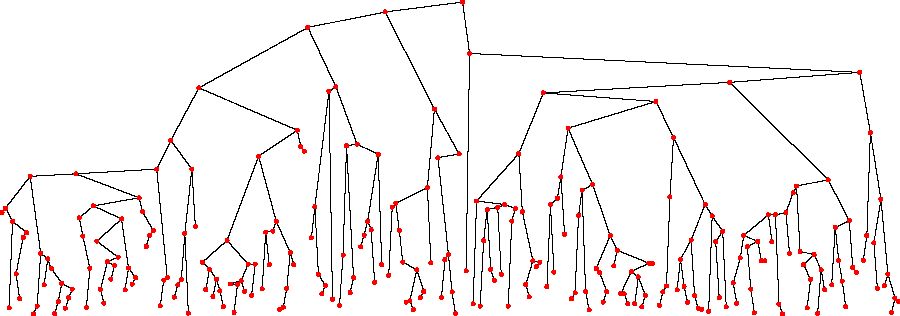
\includegraphics[scale=0.90909]{images/tree3-thick}\end{center}
  \maketitle
}}
\thetitlepage

\cleardoublepage
%
%% blank page behind title page
%\ \thispagestyle{empty}\newpage
%
%\setcounter{page}{1}
%\chapter*{Agradecimentos}
\addcontentsline{toc}{chapter}{Agradecimentos}

Sou grato a Nima~Hoda, que passou um verão corrigindo incansavelmente muitos 
dos capítulos deste livro; aos alunos da disciplina COMP2402/2002 no outono 2011, que 
aguentaram o primeiro rascunho deste livro e alertaram sobre muitos erros tipográficos, 
gramaticais e factuais; e a Morgan~Tunzelmann da Athabasca University Press, por ter 
pacientemente editado vários rascunhos quase finais.

\section{Agradecimentos da Edição Brasileira}

Gostaria de agradecer aos meus alunos do curso de Estruturas de Informação, da 
Universidade do Estado do Rio de Janeiro que gentilmente me auxiliaram na tradução
deste livro. Foram eles: Diana Almeida Barros, Ester Gomes Pais, Lucas Ferreira 
Stefe, Matheus Caldeira Matias e Pedro Yuri dos Reis de Moraes Lopes. 

Ass. João Araujo Ribeiro
%\ \thispagestyle{empty}\newpage
%\cpponly{\cpponly{
\chapter*{Preface to the C++ Edition}
\addcontentsline{toc}{chapter}{Preface to the C++ Edition}

This book is intended to teach the design and analysis of basic data
structures and their implementation in an object-oriented language.
In this edition, the language happens to be C++.

This book is not intended to act as an introduction to the C++ programming
language.  Readers of this book need only be familiar with the basic
syntax of C++ and similar languages.  Those wishing to work with the
accompanying source code should have some experience programming in C++.

This book is also not intended as an introduction to the C++ Standard
Template Library or the generic programming paradigm that the STL
embodies.  This book describes implementations of several different data
structures, many of which are used in implementations of the STL. The
contents of this book may help an STL programmer understand how some of
the STL data structures are implemented and why these implementations
are efficient.
}

%\ \thispagestyle{empty}\newpage
%}

% Use 14pt between lines
\setlength{\baselineskip}{14pt}


%\begin{titlepage}
%\maketitle
%\end{titlepage}

%\pagestyle{empty}
%half title page
%\newpage
%
%series page
%\newpage
%
%title page
%\newpage

\addtocontents{toc}{\protect\thispagestyle{empty}} % get rid of page number
\tableofcontents
\cleardoublepage

\fancyhead[RO,LE]{} % disable section numbers, for now
\pagestyle{fancy}
\chapter*{Agradecimentos}
\addcontentsline{toc}{chapter}{Agradecimentos}

Sou grato a Nima~Hoda, que passou um verão corrigindo incansavelmente muitos 
dos capítulos deste livro; aos alunos da disciplina COMP2402/2002 no outono 2011, que 
aguentaram o primeiro rascunho deste livro e alertaram sobre muitos erros tipográficos, 
gramaticais e factuais; e a Morgan~Tunzelmann da Athabasca University Press, por ter 
pacientemente editado vários rascunhos quase finais.

\section{Agradecimentos da Edição Brasileira}

Gostaria de agradecer aos meus alunos do curso de Estruturas de Informação, da 
Universidade do Estado do Rio de Janeiro que gentilmente me auxiliaram na tradução
deste livro. Foram eles: Diana Almeida Barros, Leonardo Lobão, Ester Gomes Pais, 
Fábio Cavallari, Lucas Ferreira Stefe, Matheus Caldeira Matias e Pedro Yuri 
dos Reis de Moraes Lopes. 

Ass. João Araujo Ribeiro
\thispagestyle{empty}
\cleardoublepage

\fancyhead[CE]{\small Por que este livro?} % chapter title, left center
\chapter*{Por que este Livro?}
\addcontentsline{toc}{chapter}{Por que este Livro?}

Há uma abundância de livros que ensinam estruturas introdutórias de dados.
Alguns deles são muito bons. A maioria deles custa caro, e a grande 
maioria dos estudantes de graduação em ciência da computação 
desembolsará pelo menos algum dinheiro em um livro de estruturas 
de dados.

Vários livros de código aberto de estruturas de dados estão disponíveis on-line. Alguns são muito bons, mas a maioria deles estão ficando velhos. A maioria desses livros tornaram-se gratuitos quando seus autores e/ou editores decidiram parar de atualizá-los. A atualização desses livros geralmente não é possível, por duas razões: (1)~O copyright pertence ao autor e/ou editor, qualquer um dos quais não pode permitir. (2)~O \emph{código fonte} para esses livros muitas vezes não está disponível. Ou seja, o Word, WordPerfect, FrameMaker ou fonte \LaTeX\ para o livro não está disponível, e até mesmo a versão do software que manipula essa fonte pode não estar disponível.

O objetivo deste projeto é liberar estudantes de ciência da computação de graduação de ter que pagar por um livro introdutório de estruturas de dados.
Decidi implementar este objetivo tratando este livro como um projeto de software Open Source
\index{Open Source}. 
Os scripts do fonte em \LaTeX, fontes em \lang\ e de construção para o livro estão disponíveis para download no site do autor\footnote{\url{http://opendatastructures.org}} e também, mais importante, em uma fonte confiável de gerenciamento de código.\footnote{\url{https://github.com/patmorin/ods}}

O código-fonte no site é disponível sob uma licença Creative Commons Attribution, o que significa que qualquer pessoa é livre para \emph{compartilhar}:
\index{share} para copiar, distribuir e transmitir a obra; e para \emph{remixar}:
\index{remix} 
para adaptar o trabalho, incluindo o direito de fazer uso comercial da obra. A única condição para esses direitos é a \emph{atribuição}: você deve reconhecer que o trabalho derivado contém código e/ou texto de \url{opendatastructures.org}.

Qualquer um pode contribuir com correções usando o sistema de gerenciamento de código-fonte \texttt{git}.
\index{git@\texttt{git}}
Qualquer pessoa pode também derivar fontes do livro para desenvolver uma versão separada (por exemplo, em outra linguagem de programação).
Minha esperança é que, fazendo as coisas desta maneira, este livro continue a ser um livro de texto útil muito depois de terminar meu interesse no projeto, ou meu pulso,
(o que ocorrer primeiro).




\cleardoublepage

\cpponly{
  \cpponly{
\chapter*{Preface to the C++ Edition}
\addcontentsline{toc}{chapter}{Preface to the C++ Edition}

This book is intended to teach the design and analysis of basic data
structures and their implementation in an object-oriented language.
In this edition, the language happens to be C++.

This book is not intended to act as an introduction to the C++ programming
language.  Readers of this book need only be familiar with the basic
syntax of C++ and similar languages.  Those wishing to work with the
accompanying source code should have some experience programming in C++.

This book is also not intended as an introduction to the C++ Standard
Template Library or the generic programming paradigm that the STL
embodies.  This book describes implementations of several different data
structures, many of which are used in implementations of the STL. The
contents of this book may help an STL programmer understand how some of
the STL data structures are implemented and why these implementations
are efficient.
}

  \cleardoublepage
}

\fancyhead[CE]{\small\nouppercase{\leftmark}} % chapter title, left center
\fancyhead[CO]{\small\rightmarktitle} % section title, right center
%comentei \fancyhead[RO,LE]{\small\rightmarksection} 

%% Include all the chapters one at a time
\include{intro-ptbr-lang}
\include{arrays-ptbr-lang}
\include{linkedlists-ptbr-lang}
\include{skiplists-ptbr-lang}
\include{hashing-ptbr-lang}
\include{binarytrees-ptbr-lang}
\include{rbs-ptbr-lang}
\include{scapegoat-ptbr-lang}
\include{redblack-ptbr-lang}
\include{heaps-ptbr-lang}
\include{sorting-ptbr-lang}
\include{graphs-ptbr-lang}
\include{integers-ptbr-lang}
\include{btree-ptbr-lang}

%% Turn off section numbers for remainder of document
\fancyhead[RO]{} % section number on the outside
\fancyhead[LE]{} % section number on the outside
\renewcommand{\chaptermark}[1]{\markboth{#1}{}} 
\renewcommand{\sectionmark}[1]{\markright{#1}} 
\fancyhead[CO]{\small\nouppercase\rightmark}

\cleardoublepage
\addcontentsline{toc}{chapter}{Bibliography}
\bibliographystyle{abbrvurl}
\bibliography{ods,odsproc}

\cleardoublepage
\addcontentsline{toc}{chapter}{Index}
\printindex

\end{document}

